\documentclass[aspectratio=169,11pt]{beamer}
% =====================================================================
%  pds-beamer.tex — Estilo común de las transparencias.
%
%  Uso (desde teoría/Tx/transparencias/):
%     \documentclass[aspectratio=169,11pt]{beamer}
%     % =====================================================================
%  pds-beamer.tex — Estilo común de las transparencias.
%
%  Uso (desde teoría/Tx/transparencias/):
%     \documentclass[aspectratio=169,11pt]{beamer}
%     % =====================================================================
%  pds-beamer.tex — Estilo común de las transparencias.
%
%  Uso (desde teoría/Tx/transparencias/):
%     \documentclass[aspectratio=169,11pt]{beamer}
%     \input{../../comun/pds-beamer}
%     \title{...}  \subtitle{Tema x · ...}
%     \begin{document}
%       \portada
%       ...
%     \end{document}
%  Compilar con:  latexmk -xelatex  (o «make» desde teoría/)
% =====================================================================

\usetheme{Boadilla}
\usecolortheme{orchid}
\usefonttheme{professionalfonts}
\setbeamercovered{transparent}
\setbeamersize{text margin left=0.8cm, text margin right=0.8cm}
\setbeamertemplate{navigation symbols}{}
\setbeamertemplate{itemize item}[square]
\setbeamertemplate{itemize subitem}[circle]
\setbeamertemplate{itemize subsubitem}[triangle]
\setbeamertemplate{enumerate item}[square]
\setbeamertemplate{enumerate subitem}[circle]
\setbeamertemplate{caption}{\raggedright\insertcaption\par}

\input{../../comun/pds-comun.tex}

% Tipografía: Fira Sans + Fira Math (legibles en proyector)
\usepackage{fontspec}
\usepackage{unicode-math}
% Se cargan por nombre de fichero para que funcionen con cualquier
% instalación de TeX Live (o MiKTeX) sin instalar fuentes en el sistema.
\setmainfont{FiraSans}[Extension=.otf, UprightFont=*-Regular, BoldFont=*-SemiBold,
  ItalicFont=*-Italic, BoldItalicFont=*-SemiBoldItalic]
\setsansfont{FiraSans}[Extension=.otf, UprightFont=*-Regular, BoldFont=*-SemiBold,
  ItalicFont=*-Italic, BoldItalicFont=*-SemiBoldItalic]
\setmonofont{FiraMono}[Extension=.otf, UprightFont=*-Regular, BoldFont=*-Medium, AutoFakeSlant=0.15, Scale=0.92]
\setmathfont{FiraMath-Regular.otf}
\setmathfont{latinmodern-math.otf}[range={"229B,"22EE,"22F1}]

% Colores del tema ajustados a la paleta común (más contraste)
\setbeamercolor{structure}{fg=pdsazul}
\setbeamercolor{alerted text}{fg=pdsrojo}
\setbeamercolor{example text}{fg=pdsverde}
\setbeamercolor{block title}{bg=pdsazul, fg=white}
\setbeamercolor{block body}{bg=pdsfondo}
\setbeamercolor{block title alerted}{bg=pdsrojo, fg=white}
\setbeamercolor{block body alerted}{bg=pdsrojo!6}
\setbeamercolor{block title example}{bg=pdsverde, fg=white}
\setbeamercolor{block body example}{bg=pdsverde!6}
\setbeamercolor{frametitle}{fg=pdsazul, bg=white}
\setbeamerfont{frametitle}{size=\large, series=\bfseries}
\setbeamerfont{block title}{size=\normalsize, series=\bfseries}
\setbeamertemplate{blocks}[rounded][shadow=false]

% Logo en la esquina superior derecha de cada transparencia
\pgfdeclareimage[height=0.8cm]{logo}{../../comun/ucm.png}
\addtobeamertemplate{frametitle}{}{%
  \begin{tikzpicture}[remember picture, overlay]
    \node[anchor=north east, inner sep=0pt] at ([xshift=-0.25cm, yshift=-0.2cm]current page.north east) {\pgfuseimage{logo}};
  \end{tikzpicture}}

% Datos de portada
\author[\autorescorto]{\autores}
\institute[UCM]{\footnotesize\departamento\\\universidad}
\date[\curso]{\footnotesize\grado\\\curso}

\newcommand{\portada}{%
  \begin{frame}[plain]
    \begin{center}
      
\includegraphics[height=1.9cm]{../../comun/ucm.png}
    \end{center}
    \vspace{-0.4cm}
    \titlepage
  \end{frame}}

% Índice al empezar cada sección
\AtBeginSection[]{%
  \begin{frame}{Contenido}
    \tableofcontents[currentsection, hideothersubsections]
  \end{frame}}

\renewcommand{\pdscodesize}{\scriptsize}

% Utilidades
% \herramienta{T1-convolucion-continua}: enlace a la página publicada de
% herramientas/html (se abre en el navegador, sin instalar nada).
% \herramientaservidor{server/....py}: app que necesita Python (bokeh serve).
\newcommand{\urlherramientas}{https://ucm-237.github.io/PdS/}
\newcommand{\herramienta}[1]{%
  \par\vfill\hfill{\scriptsize\color{pdsgris}\faIcon\ \href{\urlherramientas#1.html}{Herramienta interactiva: \texttt{#1}}}}
\newcommand{\herramientaservidor}[1]{%
  \par\vfill\hfill{\scriptsize\color{pdsgris}\faIcon\ Herramienta interactiva (con Python): \texttt{herramientas/#1}}}
\newcommand{\faIcon}{\textbf{▶}}
\newcommand{\gris}[1]{{\color{pdsgris}#1}}
\newcommand{\nota}[1]{\par\vspace{2pt}{\footnotesize\color{pdsgris}\textit{#1}}\par}
% Nota sobre una errata de versiones anteriores (solo con \ERRATAS)
\newcommand{\errata}[1]{\iferratas\nota{Errata de versiones anteriores: #1}\fi}
\newcommand{\apuntes}[1]{\nota{Más detalle en los apuntes, #1.}}

% Bloques con nombre en castellano
\newenvironment{definicion}[1][Definición]{\begin{block}{#1}}{\end{block}}
\newenvironment{importante}[1][Importante]{\begin{alertblock}{#1}}{\end{alertblock}}
\newenvironment{ejemplo}[1][Ejemplo]{\begin{exampleblock}{#1}}{\end{exampleblock}}

%     \title{...}  \subtitle{Tema x · ...}
%     \begin{document}
%       \portada
%       ...
%     \end{document}
%  Compilar con:  latexmk -xelatex  (o «make» desde teoría/)
% =====================================================================

\usetheme{Boadilla}
\usecolortheme{orchid}
\usefonttheme{professionalfonts}
\setbeamercovered{transparent}
\setbeamersize{text margin left=0.8cm, text margin right=0.8cm}
\setbeamertemplate{navigation symbols}{}
\setbeamertemplate{itemize item}[square]
\setbeamertemplate{itemize subitem}[circle]
\setbeamertemplate{itemize subsubitem}[triangle]
\setbeamertemplate{enumerate item}[square]
\setbeamertemplate{enumerate subitem}[circle]
\setbeamertemplate{caption}{\raggedright\insertcaption\par}

% =====================================================================
%  pds-comun.tex — Paquetes, colores y estilos de código comunes a
%  transparencias, apuntes y hojas de ejercicios. Compilar con XeLaTeX.
%  No cargar directamente: lo cargan pds-beamer.tex y pds-apuntes.tex.
% =====================================================================

\usepackage{polyglossia}
\setmainlanguage{spanish}
\usepackage{mathtools}
\usepackage{graphicx}
\usepackage{booktabs}
\usepackage{multirow}
\usepackage{array}
\usepackage{xcolor}
\usepackage{tikz}
\usetikzlibrary{positioning,arrows.meta,calc,shapes.geometric,decorations.pathreplacing}
\usepackage{listings}
\usepackage{siunitx}
\sisetup{output-decimal-marker={,}, group-separator={\,}, per-mode=symbol}

% Notas de erratas de versiones anteriores: no se imprimen salvo que se
% defina \ERRATAS antes de cargar el estilo (make ERRATAS=1)
\newif\iferratas
\ifdefined\ERRATAS \erratastrue \fi

% Ruta común (logo y figuras compartidas)
\providecommand{\rutacomun}{../../comun/}
\input{\rutacomun datos.tex}

% ---------------------------------------------------------------------
%  Paleta (la misma que usan las figuras generadas con Python,
%  ver comun/pds_estilo.py)
% ---------------------------------------------------------------------
\definecolor{pdsazul}{HTML}{2B3A8C}
\definecolor{pdsrojo}{HTML}{C0392B}
\definecolor{pdsverde}{HTML}{1E7B4F}
\definecolor{pdsnaranja}{HTML}{D9822B}
\definecolor{pdsgris}{HTML}{5A5A66}
\definecolor{pdsfondo}{HTML}{F3F4FA}
\definecolor{pdscodigo}{HTML}{F7F7F2}

% ---------------------------------------------------------------------
%  Diagramas de bloques (TikZ)
% ---------------------------------------------------------------------
\tikzset{
  bloque/.style={rectangle, rounded corners=2pt, draw=pdsazul!80, fill=pdsfondo,
                 very thick, minimum height=8mm, minimum width=14mm, align=center},
  sumador/.style={circle, draw=pdsazul!80, fill=pdsfondo, thick, inner sep=1.5pt},
  flecha/.style={-{Stealth[length=2.2mm]}, thick, pdsgris},
}

% ---------------------------------------------------------------------
%  Código: Python y Matlab en paralelo
% ---------------------------------------------------------------------
\newcommand{\pdscodesize}{\footnotesize}
\lstdefinestyle{pds}{
  basicstyle=\ttfamily\pdscodesize,
  keywordstyle=\color{pdsazul}\bfseries,
  commentstyle=\color{pdsverde}\itshape,
  stringstyle=\color{pdsrojo},
  numbers=none,
  backgroundcolor=\color{pdscodigo},
  frame=single, rulecolor=\color{pdsgris!40}, framerule=0.4pt,
  xleftmargin=2pt, xrightmargin=2pt, aboveskip=2pt, belowskip=2pt,
  columns=fullflexible, keepspaces=true,
  showstringspaces=false, breaklines=true, tabsize=4,
  upquote=true,
  % Con XeLaTeX, listings desordena los caracteres no ASCII junto a
  % dígitos («2π» sale «π2»): se sustituyen por su versión matemática.
  literate={π}{{$\pi$}}1 {δ}{{$\delta$}}1 {ω}{{$\omega$}}1 {Ω}{{$\Omega$}}1
           {≈}{{$\approx$}}1 {µ}{{$\mu$}}1 {·}{{$\cdot$}}1 {α}{{$\alpha$}}1
           {á}{{á}}1 {é}{{é}}1 {í}{{í}}1 {ó}{{ó}}1 {ú}{{ú}}1 {ñ}{{ñ}}1 {¿}{{¿}}1,
}
\lstdefinestyle{python}{style=pds, language=Python,
  morekeywords={as,True,False,None}}
\lstdefinestyle{matlab}{style=pds, language=Matlab,
  morekeywords={function,end,true,false}}

% \codigo{<ruta sin extensión>} muestra el mismo ejemplo en Python
% y en Matlab, uno al lado del otro. Los ficheros viven en
% ../codigo/python/<nombre>.py y ../codigo/matlab/<nombre>.m y se
% ejecutan en las pruebas (make prueba-codigo).
\newcommand{\rutacodigo}{../codigo/}
\newcommand{\codigoetiqueta}[1]{{\sffamily\scriptsize\bfseries\color{pdsgris}#1}}
\newcommand{\codigo}[2][]{%
  \par\noindent
  \begin{minipage}[t]{0.495\linewidth}
    \codigoetiqueta{Python}\par\vspace{1pt}
    \lstinputlisting[style=python,#1]{\rutacodigo python/#2.py}
  \end{minipage}\hfill
  \begin{minipage}[t]{0.495\linewidth}
    \codigoetiqueta{Matlab}\par\vspace{1pt}
    \lstinputlisting[style=matlab,#1]{\rutacodigo matlab/#2.m}
  \end{minipage}\par}

\input{\rutacomun notacion.tex}


% Tipografía: Fira Sans + Fira Math (legibles en proyector)
\usepackage{fontspec}
\usepackage{unicode-math}
% Se cargan por nombre de fichero para que funcionen con cualquier
% instalación de TeX Live (o MiKTeX) sin instalar fuentes en el sistema.
\setmainfont{FiraSans}[Extension=.otf, UprightFont=*-Regular, BoldFont=*-SemiBold,
  ItalicFont=*-Italic, BoldItalicFont=*-SemiBoldItalic]
\setsansfont{FiraSans}[Extension=.otf, UprightFont=*-Regular, BoldFont=*-SemiBold,
  ItalicFont=*-Italic, BoldItalicFont=*-SemiBoldItalic]
\setmonofont{FiraMono}[Extension=.otf, UprightFont=*-Regular, BoldFont=*-Medium, AutoFakeSlant=0.15, Scale=0.92]
\setmathfont{FiraMath-Regular.otf}
\setmathfont{latinmodern-math.otf}[range={"229B,"22EE,"22F1}]

% Colores del tema ajustados a la paleta común (más contraste)
\setbeamercolor{structure}{fg=pdsazul}
\setbeamercolor{alerted text}{fg=pdsrojo}
\setbeamercolor{example text}{fg=pdsverde}
\setbeamercolor{block title}{bg=pdsazul, fg=white}
\setbeamercolor{block body}{bg=pdsfondo}
\setbeamercolor{block title alerted}{bg=pdsrojo, fg=white}
\setbeamercolor{block body alerted}{bg=pdsrojo!6}
\setbeamercolor{block title example}{bg=pdsverde, fg=white}
\setbeamercolor{block body example}{bg=pdsverde!6}
\setbeamercolor{frametitle}{fg=pdsazul, bg=white}
\setbeamerfont{frametitle}{size=\large, series=\bfseries}
\setbeamerfont{block title}{size=\normalsize, series=\bfseries}
\setbeamertemplate{blocks}[rounded][shadow=false]

% Logo en la esquina superior derecha de cada transparencia
\pgfdeclareimage[height=0.8cm]{logo}{../../comun/ucm.png}
\addtobeamertemplate{frametitle}{}{%
  \begin{tikzpicture}[remember picture, overlay]
    \node[anchor=north east, inner sep=0pt] at ([xshift=-0.25cm, yshift=-0.2cm]current page.north east) {\pgfuseimage{logo}};
  \end{tikzpicture}}

% Datos de portada
\author[\autorescorto]{\autores}
\institute[UCM]{\footnotesize\departamento\\\universidad}
\date[\curso]{\footnotesize\grado\\\curso}

\newcommand{\portada}{%
  \begin{frame}[plain]
    \begin{center}
      
\includegraphics[height=1.9cm]{../../comun/ucm.png}
    \end{center}
    \vspace{-0.4cm}
    \titlepage
  \end{frame}}

% Índice al empezar cada sección
\AtBeginSection[]{%
  \begin{frame}{Contenido}
    \tableofcontents[currentsection, hideothersubsections]
  \end{frame}}

\renewcommand{\pdscodesize}{\scriptsize}

% Utilidades
% \herramienta{T1-convolucion-continua}: enlace a la página publicada de
% herramientas/html (se abre en el navegador, sin instalar nada).
% \herramientaservidor{server/....py}: app que necesita Python (bokeh serve).
\newcommand{\urlherramientas}{https://ucm-237.github.io/PdS/}
\newcommand{\herramienta}[1]{%
  \par\vfill\hfill{\scriptsize\color{pdsgris}\faIcon\ \href{\urlherramientas#1.html}{Herramienta interactiva: \texttt{#1}}}}
\newcommand{\herramientaservidor}[1]{%
  \par\vfill\hfill{\scriptsize\color{pdsgris}\faIcon\ Herramienta interactiva (con Python): \texttt{herramientas/#1}}}
\newcommand{\faIcon}{\textbf{▶}}
\newcommand{\gris}[1]{{\color{pdsgris}#1}}
\newcommand{\nota}[1]{\par\vspace{2pt}{\footnotesize\color{pdsgris}\textit{#1}}\par}
% Nota sobre una errata de versiones anteriores (solo con \ERRATAS)
\newcommand{\errata}[1]{\iferratas\nota{Errata de versiones anteriores: #1}\fi}
\newcommand{\apuntes}[1]{\nota{Más detalle en los apuntes, #1.}}

% Bloques con nombre en castellano
\newenvironment{definicion}[1][Definición]{\begin{block}{#1}}{\end{block}}
\newenvironment{importante}[1][Importante]{\begin{alertblock}{#1}}{\end{alertblock}}
\newenvironment{ejemplo}[1][Ejemplo]{\begin{exampleblock}{#1}}{\end{exampleblock}}

%     \title{...}  \subtitle{Tema x · ...}
%     \begin{document}
%       \portada
%       ...
%     \end{document}
%  Compilar con:  latexmk -xelatex  (o «make» desde teoría/)
% =====================================================================

\usetheme{Boadilla}
\usecolortheme{orchid}
\usefonttheme{professionalfonts}
\setbeamercovered{transparent}
\setbeamersize{text margin left=0.8cm, text margin right=0.8cm}
\setbeamertemplate{navigation symbols}{}
\setbeamertemplate{itemize item}[square]
\setbeamertemplate{itemize subitem}[circle]
\setbeamertemplate{itemize subsubitem}[triangle]
\setbeamertemplate{enumerate item}[square]
\setbeamertemplate{enumerate subitem}[circle]
\setbeamertemplate{caption}{\raggedright\insertcaption\par}

% =====================================================================
%  pds-comun.tex — Paquetes, colores y estilos de código comunes a
%  transparencias, apuntes y hojas de ejercicios. Compilar con XeLaTeX.
%  No cargar directamente: lo cargan pds-beamer.tex y pds-apuntes.tex.
% =====================================================================

\usepackage{polyglossia}
\setmainlanguage{spanish}
\usepackage{mathtools}
\usepackage{graphicx}
\usepackage{booktabs}
\usepackage{multirow}
\usepackage{array}
\usepackage{xcolor}
\usepackage{tikz}
\usetikzlibrary{positioning,arrows.meta,calc,shapes.geometric,decorations.pathreplacing}
\usepackage{listings}
\usepackage{siunitx}
\sisetup{output-decimal-marker={,}, group-separator={\,}, per-mode=symbol}

% Notas de erratas de versiones anteriores: no se imprimen salvo que se
% defina \ERRATAS antes de cargar el estilo (make ERRATAS=1)
\newif\iferratas
\ifdefined\ERRATAS \erratastrue \fi

% Ruta común (logo y figuras compartidas)
\providecommand{\rutacomun}{../../comun/}
\input{\rutacomun datos.tex}

% ---------------------------------------------------------------------
%  Paleta (la misma que usan las figuras generadas con Python,
%  ver comun/pds_estilo.py)
% ---------------------------------------------------------------------
\definecolor{pdsazul}{HTML}{2B3A8C}
\definecolor{pdsrojo}{HTML}{C0392B}
\definecolor{pdsverde}{HTML}{1E7B4F}
\definecolor{pdsnaranja}{HTML}{D9822B}
\definecolor{pdsgris}{HTML}{5A5A66}
\definecolor{pdsfondo}{HTML}{F3F4FA}
\definecolor{pdscodigo}{HTML}{F7F7F2}

% ---------------------------------------------------------------------
%  Diagramas de bloques (TikZ)
% ---------------------------------------------------------------------
\tikzset{
  bloque/.style={rectangle, rounded corners=2pt, draw=pdsazul!80, fill=pdsfondo,
                 very thick, minimum height=8mm, minimum width=14mm, align=center},
  sumador/.style={circle, draw=pdsazul!80, fill=pdsfondo, thick, inner sep=1.5pt},
  flecha/.style={-{Stealth[length=2.2mm]}, thick, pdsgris},
}

% ---------------------------------------------------------------------
%  Código: Python y Matlab en paralelo
% ---------------------------------------------------------------------
\newcommand{\pdscodesize}{\footnotesize}
\lstdefinestyle{pds}{
  basicstyle=\ttfamily\pdscodesize,
  keywordstyle=\color{pdsazul}\bfseries,
  commentstyle=\color{pdsverde}\itshape,
  stringstyle=\color{pdsrojo},
  numbers=none,
  backgroundcolor=\color{pdscodigo},
  frame=single, rulecolor=\color{pdsgris!40}, framerule=0.4pt,
  xleftmargin=2pt, xrightmargin=2pt, aboveskip=2pt, belowskip=2pt,
  columns=fullflexible, keepspaces=true,
  showstringspaces=false, breaklines=true, tabsize=4,
  upquote=true,
  % Con XeLaTeX, listings desordena los caracteres no ASCII junto a
  % dígitos («2π» sale «π2»): se sustituyen por su versión matemática.
  literate={π}{{$\pi$}}1 {δ}{{$\delta$}}1 {ω}{{$\omega$}}1 {Ω}{{$\Omega$}}1
           {≈}{{$\approx$}}1 {µ}{{$\mu$}}1 {·}{{$\cdot$}}1 {α}{{$\alpha$}}1
           {á}{{á}}1 {é}{{é}}1 {í}{{í}}1 {ó}{{ó}}1 {ú}{{ú}}1 {ñ}{{ñ}}1 {¿}{{¿}}1,
}
\lstdefinestyle{python}{style=pds, language=Python,
  morekeywords={as,True,False,None}}
\lstdefinestyle{matlab}{style=pds, language=Matlab,
  morekeywords={function,end,true,false}}

% \codigo{<ruta sin extensión>} muestra el mismo ejemplo en Python
% y en Matlab, uno al lado del otro. Los ficheros viven en
% ../codigo/python/<nombre>.py y ../codigo/matlab/<nombre>.m y se
% ejecutan en las pruebas (make prueba-codigo).
\newcommand{\rutacodigo}{../codigo/}
\newcommand{\codigoetiqueta}[1]{{\sffamily\scriptsize\bfseries\color{pdsgris}#1}}
\newcommand{\codigo}[2][]{%
  \par\noindent
  \begin{minipage}[t]{0.495\linewidth}
    \codigoetiqueta{Python}\par\vspace{1pt}
    \lstinputlisting[style=python,#1]{\rutacodigo python/#2.py}
  \end{minipage}\hfill
  \begin{minipage}[t]{0.495\linewidth}
    \codigoetiqueta{Matlab}\par\vspace{1pt}
    \lstinputlisting[style=matlab,#1]{\rutacodigo matlab/#2.m}
  \end{minipage}\par}

\input{\rutacomun notacion.tex}


% Tipografía: Fira Sans + Fira Math (legibles en proyector)
\usepackage{fontspec}
\usepackage{unicode-math}
% Se cargan por nombre de fichero para que funcionen con cualquier
% instalación de TeX Live (o MiKTeX) sin instalar fuentes en el sistema.
\setmainfont{FiraSans}[Extension=.otf, UprightFont=*-Regular, BoldFont=*-SemiBold,
  ItalicFont=*-Italic, BoldItalicFont=*-SemiBoldItalic]
\setsansfont{FiraSans}[Extension=.otf, UprightFont=*-Regular, BoldFont=*-SemiBold,
  ItalicFont=*-Italic, BoldItalicFont=*-SemiBoldItalic]
\setmonofont{FiraMono}[Extension=.otf, UprightFont=*-Regular, BoldFont=*-Medium, AutoFakeSlant=0.15, Scale=0.92]
\setmathfont{FiraMath-Regular.otf}
\setmathfont{latinmodern-math.otf}[range={"229B,"22EE,"22F1}]

% Colores del tema ajustados a la paleta común (más contraste)
\setbeamercolor{structure}{fg=pdsazul}
\setbeamercolor{alerted text}{fg=pdsrojo}
\setbeamercolor{example text}{fg=pdsverde}
\setbeamercolor{block title}{bg=pdsazul, fg=white}
\setbeamercolor{block body}{bg=pdsfondo}
\setbeamercolor{block title alerted}{bg=pdsrojo, fg=white}
\setbeamercolor{block body alerted}{bg=pdsrojo!6}
\setbeamercolor{block title example}{bg=pdsverde, fg=white}
\setbeamercolor{block body example}{bg=pdsverde!6}
\setbeamercolor{frametitle}{fg=pdsazul, bg=white}
\setbeamerfont{frametitle}{size=\large, series=\bfseries}
\setbeamerfont{block title}{size=\normalsize, series=\bfseries}
\setbeamertemplate{blocks}[rounded][shadow=false]

% Logo en la esquina superior derecha de cada transparencia
\pgfdeclareimage[height=0.8cm]{logo}{../../comun/ucm.png}
\addtobeamertemplate{frametitle}{}{%
  \begin{tikzpicture}[remember picture, overlay]
    \node[anchor=north east, inner sep=0pt] at ([xshift=-0.25cm, yshift=-0.2cm]current page.north east) {\pgfuseimage{logo}};
  \end{tikzpicture}}

% Datos de portada
\author[\autorescorto]{\autores}
\institute[UCM]{\footnotesize\departamento\\\universidad}
\date[\curso]{\footnotesize\grado\\\curso}

\newcommand{\portada}{%
  \begin{frame}[plain]
    \begin{center}
      
\includegraphics[height=1.9cm]{../../comun/ucm.png}
    \end{center}
    \vspace{-0.4cm}
    \titlepage
  \end{frame}}

% Índice al empezar cada sección
\AtBeginSection[]{%
  \begin{frame}{Contenido}
    \tableofcontents[currentsection, hideothersubsections]
  \end{frame}}

\renewcommand{\pdscodesize}{\scriptsize}

% Utilidades
% \herramienta{T1-convolucion-continua}: enlace a la página publicada de
% herramientas/html (se abre en el navegador, sin instalar nada).
% \herramientaservidor{server/....py}: app que necesita Python (bokeh serve).
\newcommand{\urlherramientas}{https://ucm-237.github.io/PdS/}
\newcommand{\herramienta}[1]{%
  \par\vfill\hfill{\scriptsize\color{pdsgris}\faIcon\ \href{\urlherramientas#1.html}{Herramienta interactiva: \texttt{#1}}}}
\newcommand{\herramientaservidor}[1]{%
  \par\vfill\hfill{\scriptsize\color{pdsgris}\faIcon\ Herramienta interactiva (con Python): \texttt{herramientas/#1}}}
\newcommand{\faIcon}{\textbf{▶}}
\newcommand{\gris}[1]{{\color{pdsgris}#1}}
\newcommand{\nota}[1]{\par\vspace{2pt}{\footnotesize\color{pdsgris}\textit{#1}}\par}
% Nota sobre una errata de versiones anteriores (solo con \ERRATAS)
\newcommand{\errata}[1]{\iferratas\nota{Errata de versiones anteriores: #1}\fi}
\newcommand{\apuntes}[1]{\nota{Más detalle en los apuntes, #1.}}

% Bloques con nombre en castellano
\newenvironment{definicion}[1][Definición]{\begin{block}{#1}}{\end{block}}
\newenvironment{importante}[1][Importante]{\begin{alertblock}{#1}}{\end{alertblock}}
\newenvironment{ejemplo}[1][Ejemplo]{\begin{exampleblock}{#1}}{\end{exampleblock}}

\graphicspath{{../figuras/}}

\title[T5 · Imágenes]{Aplicaciones}
\subtitle{Tema 5 · Parte 3: procesamiento de imágenes}

\begin{document}
\portada

% =====================================================================
\section{La imagen como señal 2D}

\begin{frame}{Imagen digital}
  \begin{center}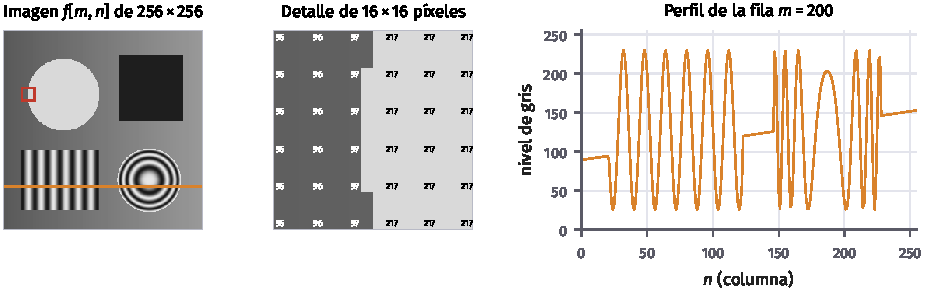
\includegraphics[width=0.85\linewidth]{imagen_pixeles}\end{center}
  \small
  \begin{itemize}
    \item Una imagen es una señal de \alert{dos variables espaciales}. Muestreada y cuantificada es una matriz $f[m,n]$ de $M\times N$ \alert{píxeles}: $m$ es la fila (hacia abajo) y $n$ la columna.
    \item Escala de grises: un valor por píxel, normalmente entero de 8 bits (0 negro, 255 blanco) o real en $[0,1]$.
    \item Color: tres canales (rojo, verde, azul), una matriz de $M\times N\times3$.
  \end{itemize}
\end{frame}

\begin{frame}{Muestreo, cuantificación y almacenamiento}
  \footnotesize
  \begin{itemize}
    \item \alert{Muestreo espacial}: el sensor toma muestras con un paso $\Delta x$; la frecuencia espacial se mide en ciclos por píxel (o por milímetro). Si la escena tiene detalles más finos que $2\Delta x$ aparece \alert{aliasing}: el efecto moiré de una camisa a rayas.
    \item \alert{Cuantificación}: con $b$ bits hay $2^b$ niveles. Con pocos niveles aparecen contornos falsos en los degradados.
    \item \alert{Tamaño}: $M\cdot N\cdot(\text{canales})\cdot b/8$ bytes. Una imagen en color de $1920\times1080$ a 8 bits ocupa unos 6,2\,MB sin comprimir.
    \item \alert{Formatos}:
    \begin{itemize}
      \item sin compresión (\emph{raw}, BMP);
      \item compresión sin pérdidas (PNG, TIFF): eliminan redundancia;
      \item compresión con pérdidas (JPEG, JPEG 2000): descartan lo que menos se ve, con la DCT por bloques o con wavelets.
    \end{itemize}
    \item Matlab: \texttt{imread}, \texttt{imshow}, \texttt{imwrite}. Python: \texttt{matplotlib.pyplot.imread} y \texttt{imshow}, o el paquete Pillow.
  \end{itemize}
  \nota{Los ejemplos del tema usan una imagen sintética, \texttt{imagen\_prueba}, para no depender de ficheros externos.}
\end{frame}

% =====================================================================
\section{Operaciones puntuales e histograma}

\begin{frame}{Operaciones puntuales}
  \begin{center}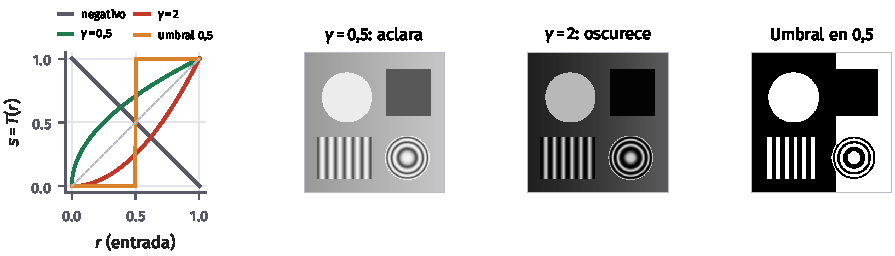
\includegraphics[width=\linewidth]{transformaciones_puntuales}\end{center}
  \small
  \begin{itemize}
    \item Cada píxel se transforma con la misma función de su valor: $s=T(r)$. No intervienen los vecinos.
    \item Negativo $s=1-r$; corrección gamma $s=r^\gamma$ ($\gamma<1$ aclara, $\gamma>1$ oscurece); estiramiento lineal de $[r_1,r_2]$ a $[0,1]$; umbralización, que da una imagen binaria.
  \end{itemize}
\end{frame}

\begin{frame}{Histograma}
  \footnotesize
  \begin{definicion}[Histograma de una imagen]
    Con $L$ niveles $r=0,\dots,L-1$, $h[r]$ es el número de píxeles con nivel $r$. Normalizado, $p[r]=h[r]/(MN)$ es la proporción de píxeles de cada nivel, y su suma acumulada
    \[
      F(r)=\sum_{i=0}^{r}p[i]
    \]
    es la función de distribución de los niveles.
  \end{definicion}
  \begin{itemize}
    \item Imagen oscura: histograma concentrado a la izquierda; clara, a la derecha; con poco contraste, estrecho.
    \item El histograma no dice dónde están los píxeles: dos imágenes muy distintas pueden tener el mismo. Es la misma idea que el histograma de muestras del tema~6.
    \item Permite elegir un \alert{umbral} para separar objeto y fondo (por ejemplo, en el valle entre dos picos; método de Otsu).
  \end{itemize}
\end{frame}

\begin{frame}{Ecualización del histograma}
  \begin{center}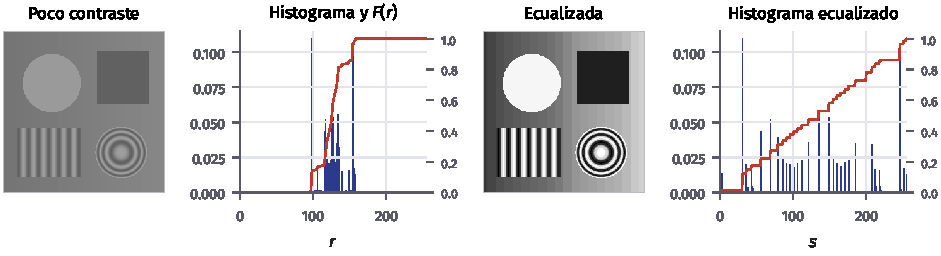
\includegraphics[width=\linewidth]{histograma_ecualizacion}\end{center}
  \small
  \begin{itemize}
    \item Se aplica la transformación $s=T(r)=\operatorname{round}\big((L-1)\,F(r)\big)$, que es creciente.
    \item Si $r$ fuera continua, $s$ tendría distribución uniforme (tema~6: la distribución aplicada a su propia variable es uniforme). Con niveles discretos el histograma no queda plano, pero se reparte por todo el rango.
  \end{itemize}
\end{frame}

\begin{frame}{En código: ecualización}
  \codigo{ecualizacion}
  \nota{La desviación típica de los niveles, una medida del contraste, pasa de 17 a 73. Con la Image Processing Toolbox: \texttt{imhist}, \texttt{histeq}, \texttt{imadjust}.}
\end{frame}

% =====================================================================
\section{Convolución 2D y filtrado espacial}

\begin{frame}{Convolución bidimensional}
  \begin{columns}[c]
    \begin{column}{0.55\textwidth}
      \small
      \begin{definicion}[Convolución 2D]
        \[
          g[m,n]=(h\conv f)[m,n]=\sum_{i}\sum_{j}h[i,j]\,f[m-i,n-j]
        \]
      \end{definicion}
      \begin{itemize}
        \item $h$ es el \alert{núcleo} (o máscara) del filtro, normalmente pequeño ($3\times3$, $5\times5$): un FIR 2D.
        \item Cada píxel de salida es una combinación de sus vecinos. Sistema lineal e invariante al desplazamiento.
        \item Imagen $M\times N$ y núcleo $K\times K$: la salida completa mide $(M+K-1)\times(N+K-1)$; con \texttt{'same'} se recorta al tamaño de la entrada.
      \end{itemize}
    \end{column}
    \begin{column}{0.42\textwidth}
      \small
      \begin{itemize}
        \item \alert{Bordes}: fuera de la imagen hay que suponer algo: ceros, repetir el borde o reflejar.
        \item \alert{Separable} si $h[i,j]=u[i]\,v[j]$: se filtran las filas con $v$ y las columnas con $u$. Cuesta $2K$ productos por píxel en vez de $K^2$.
      \end{itemize}
      \[
        \underbrace{\begin{bmatrix}1&0&-1\\2&0&-2\\1&0&-1\end{bmatrix}}_{\text{Sobel}}=\begin{bmatrix}1\\2\\1\end{bmatrix}\begin{bmatrix}1&0&-1\end{bmatrix}
      \]
    \end{column}
  \end{columns}
  \nota{\texttt{conv2} (Matlab), \texttt{convolve2d} (Python). \texttt{filter2} e \texttt{imfilter} calculan la correlación.}
\end{frame}

\begin{frame}{Núcleos habituales}
  \begin{center}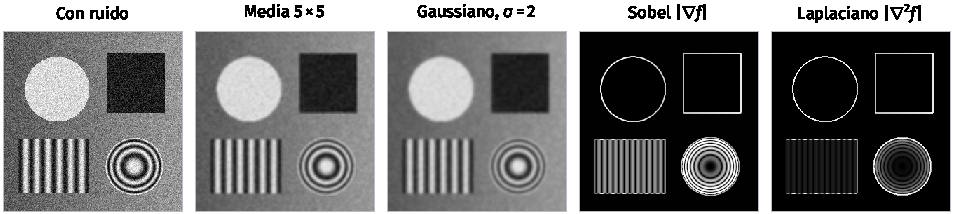
\includegraphics[width=\linewidth]{filtros_espaciales}\end{center}
  \footnotesize
  \begin{columns}[T]
    \begin{column}{0.5\textwidth}
      \begin{itemize}
        \item \alert{Paso bajo}: media $\frac1{K^2}\mathbf 1_{K\times K}$ o gaussiano $h[i,j]\propto\e^{-(i^2+j^2)/(2\sigma^2)}$. Suavizan y reducen ruido; emborronan los bordes. El gaussiano no deja artefactos.
      \end{itemize}
    \end{column}
    \begin{column}{0.5\textwidth}
      \begin{itemize}
        \item \alert{Derivadas}: Sobel aproxima $\partial f/\partial n$ y su traspuesto $\partial f/\partial m$; $\abs{\nabla f}=\sqrt{g_x^2+g_y^2}$ marca los bordes.
        \item Laplaciano $\begin{bsmallmatrix}0&1&0\\1&-4&1\\0&1&0\end{bsmallmatrix}$: segunda derivada, realza detalles y ruido.
      \end{itemize}
    \end{column}
  \end{columns}
\end{frame}

\begin{frame}{En código: bordes con Sobel}
  \codigo[basicstyle=\ttfamily\fontsize{6.8}{7.8}\selectfont]{sobel}
  \nota{En el degradado $f$ crece $0{,}25/256$ por columna y Sobel da 8 veces esa derivada.}
\end{frame}

% =====================================================================
\section{DFT bidimensional}

\begin{frame}{Definición}
  \begin{definicion}[DFT 2D de una imagen $M\times N$]
    \[
      F[k,l]=\sum_{m=0}^{M-1}\sum_{n=0}^{N-1}f[m,n]\,\e^{-j2\pi\left(\frac{km}{M}+\frac{ln}{N}\right)},\qquad
      f[m,n]=\frac1{MN}\sum_{k=0}^{M-1}\sum_{l=0}^{N-1}F[k,l]\,\e^{j2\pi\left(\frac{km}{M}+\frac{ln}{N}\right)}
    \]
  \end{definicion}
  \small
  \begin{itemize}
    \item Descompone la imagen en \alert{ondas planas} $\e^{j2\pi(km/M+ln/N)}$: franjas con $k$ ciclos en vertical y $l$ en horizontal. $F[0,0]$ es la suma de todos los píxeles.
    \item \alert{Separable}: DFT 1D de cada fila y después de cada columna. Con la FFT cuesta $O(MN\log(MN))$. Matlab y Python: \texttt{fft2}, \texttt{ifft2}.
    \item Se dibuja $\log(1+\abs{F})$ con el origen en el centro (\texttt{fftshift}), porque $\abs F$ abarca muchos órdenes de magnitud.
  \end{itemize}
\end{frame}

\begin{frame}{Ejemplos}
  \begin{columns}[c]
    \begin{column}{0.58\textwidth}
      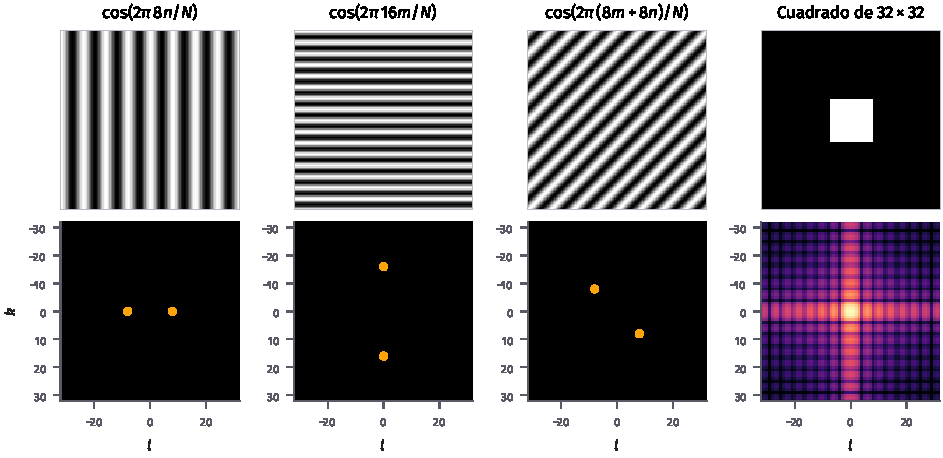
\includegraphics[width=\linewidth]{dft2_patrones}
    \end{column}
    \begin{column}{0.4\textwidth}
      \small
      \begin{itemize}
        \item Un coseno da dos puntos simétricos, en la dirección \emph{perpendicular} a las franjas.
        \item Más franjas por píxel, puntos más lejos del centro.
        \item Un cuadrado da un $\sinc$ en cada dirección (tema~3), con lóbulos en forma de cruz.
        \item Bordes rectos de la imagen producen rayas perpendiculares en la DFT.
      \end{itemize}
    \end{column}
  \end{columns}
\end{frame}

\begin{frame}{Propiedades}
  \footnotesize
  \begin{columns}[T]
    \begin{column}{0.5\textwidth}
      \begin{itemize}
        \item \alert{Periodicidad}: $F[k+M,l]=F[k,l+N]=F[k,l]$. Por eso se puede centrar con \texttt{fftshift}.
        \item \alert{Simetría}: si $f$ es real, $F[-k,-l]=F^*[k,l]$.
        \item \alert{Desplazamiento} (circular):
        \[
          f[m-m_0,n-n_0]\parF\e^{-j2\pi\left(\frac{km_0}{M}+\frac{ln_0}{N}\right)}F[k,l]:
        \]
        el módulo no cambia.
        \item \alert{Rotación}: girar la imagen gira la DFT el mismo ángulo.
      \end{itemize}
    \end{column}
    \begin{column}{0.5\textwidth}
      \begin{itemize}
        \item \alert{Convolución}: la convolución circular 2D es el producto de las DFT. Para la lineal se rellena con ceros hasta $(M+K-1)\times(N+K-1)$.
        \item \alert{Linealidad} y \alert{Parseval}: $\sum\abs{f}^2=\frac1{MN}\sum\abs{F}^2$.
      \end{itemize}
      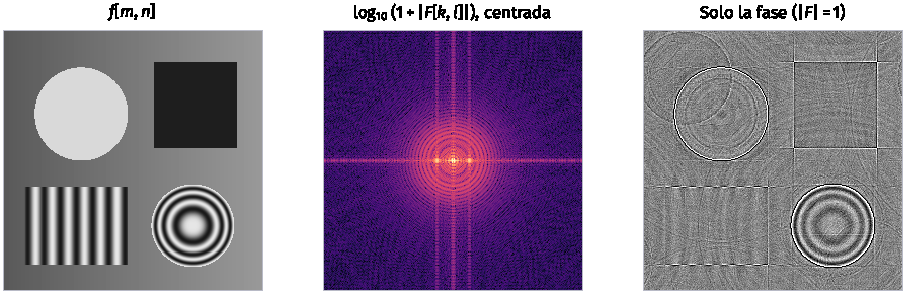
\includegraphics[width=\linewidth]{dft2_imagen}
      \nota{La fase lleva la posición de los bordes: con solo la fase se reconocen los objetos.}
    \end{column}
  \end{columns}
  \nota{Erratas antiguas: faltaban $M$ y $N$ en la propiedad de desplazamiento, y la de escalado era la de la transformada continua, que no vale para la DFT.}
\end{frame}

% =====================================================================
\section{Filtrado en frecuencia}

\begin{frame}{Filtros en el dominio de la frecuencia}
  \begin{columns}[c]
    \begin{column}{0.42\textwidth}
      \small
      \begin{itemize}
        \item $G[k,l]=H[k,l]\,F[k,l]$ y $g=\IDFT\{G\}$. Con $D[k,l]$ la distancia al origen (centrado):
        \item Ideal: $H=1$ si $D\le D_0$. Su respuesta al impulso es un $\sinc$ 2D: \alert{anillos} alrededor de los bordes.
        \item Gaussiano: $H=\e^{-D^2/(2D_0^2)}$. Equivale a convolucionar con un gaussiano de $\sigma=N/(2\pi D_0)$ píxeles.
        \item Paso alto: $1-H_{\text{PB}}$.
      \end{itemize}
    \end{column}
    \begin{column}{0.56\textwidth}
      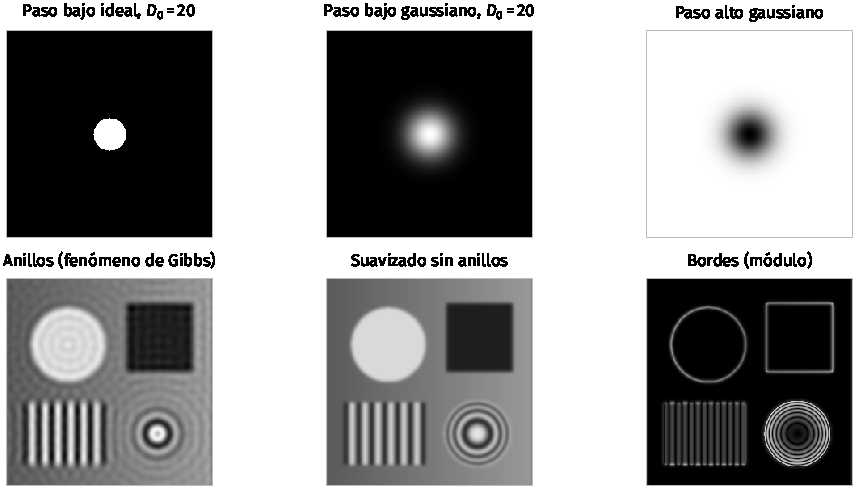
\includegraphics[width=\linewidth]{filtrado_frecuencia}
    \end{column}
  \end{columns}
\end{frame}

\begin{frame}{En código: paso bajo gaussiano con la DFT}
  \codigo{filtro_frecuencia_2d}
  \nota{$N=256$, $D_0=20$: equivale a un gaussiano espacial de $\sigma\approx2$ píxeles.}
\end{frame}

\begin{frame}{Más allá}
  \begin{itemize}
    \item \alert{Restauración}: deshacer un desenfoque conocido dividiendo por $H$ (con cuidado donde $H\approx0$: filtro de Wiener).
    \item \alert{Compresión}: JPEG aplica la DCT a bloques de $8\times8$ y cuantifica más las frecuencias altas; JPEG 2000 usa una DWT 2D.
    \item \alert{Segmentación y morfología}: umbralizar, detectar bordes, rellenar y medir objetos.
    \item \alert{Visión por computador}: las redes convolucionales encadenan muchas convoluciones 2D con núcleos aprendidos.
  \end{itemize}
\end{frame}

% =====================================================================
\section*{Resumen}
\begin{frame}{Conceptos importantes}
  \begin{columns}[T]
    \begin{column}{0.5\textwidth}
      \begin{itemize}
        \item Imagen: matriz $f[m,n]$ de $M\times N$ píxeles; uno o tres canales.
        \item Operaciones puntuales $s=T(r)$; histograma y ecualización con $T=(L-1)F$.
        \item Convolución 2D con núcleos pequeños: suavizado, Sobel, laplaciano; separabilidad.
      \end{itemize}
    \end{column}
    \begin{column}{0.5\textwidth}
      \begin{itemize}
        \item DFT 2D separable; \texttt{fftshift} y $\log(1+\abs F)$.
        \item Periodicidad, simetría, desplazamiento, rotación, convolución.
        \item Filtrado en frecuencia: el ideal produce anillos; el gaussiano no.
      \end{itemize}
    \end{column}
  \end{columns}
  \bigskip
  \gris{Apuntes del Tema 5, sección 3 · Hoja de ejercicios, ejercicios 11–16.}
\end{frame}

\end{document}
